\section{Experiments}
All timing experiments run on one MacBook (Apple silicon, macOS 26) on a campus Wi-Fi network. Root access is not used: Unbound runs on a high local port and the daemon runs unchanged against it. Network conditions are set by a local SOCKS5 proxy that adds a fixed round-trip delay per connection (10, 60 or 150\,ms, standing for home, busy campus and poor Wi-Fi) and resolves names either with the system resolver (Mac tool off) or through the local Unbound plus predictor (Mac tool on). Chrome is Chrome for Testing 159 driven by Playwright, with all host resolution forced through the proxy. Condition order is randomised per site or per round, medians and 75th percentiles are reported with bootstrap 95\% intervals (2{,}000 resamples), and $n$ is stated for every cell. Every number in this paper is read by a script from \texttt{RESULTS.md}, which is itself generated from the raw result files.

\textbf{Route 0, offline replay (kill test).} The predictor and four baselines (most popular, last successor, order-1 Markov with the same estimator, and PPM-C) replay public traces: MSNBC page categories, the NASA (July 1995) and ClarkNet (August 1995) HTTP logs, and Wikispeedia navigation paths, 1{,}000 users each, plus one recorded person's Chrome history (domains, and hashed paths per origin). Before running, the pass threshold was set: the mixture's log-loss must beat order-1 Markov with a 95\% interval below zero on most traces. The 30 users used for development were excluded.

\textbf{Route 1, lookups.} dnspyre resolves the Tranco top \V{r1.names} names, \V{r1.rounds} rounds \V{r1.wait}\,s apart, under three conditions: the network's resolver, Unbound alone with its own prefetch, and Unbound with the predictor's daemon.

\textbf{Route 2, page loads.} For each of 50 Tranco sites with a same-origin link that does not redirect, a session loads the home page, waits 1.5\,s (the time a person spends reading; the extension decides here), clicks the link, and records how long the person waited for the next page (load end minus prerender activation). Each session first visits home and the link once per DNS mode, so the extension has seen the path. The design is $2\times2$ (Mac tool, extension) at three Wi-Fi profiles; the six profile-by-extension sessions run at once, each with its own browser profile and proxy, and DNS mode order is shuffled per site.

\textbf{Route 3, API calls.} curl fetches one URL from each of \V{r3.hosts} API hosts, \V{r3.rounds} rounds, with the Mac tool off and on in shuffled order.

\section{Results}
\textbf{Route 0 passed.} The mixture's log-loss was lower than order-1 Markov's on \V{r0.wins_markov_bits} of \V{r0.ntraces} traces with the whole 95\% interval below zero, and lower than PPM-C's on \V{r0.wins_ppmc_bits} of \V{r0.ntraces} (Figure~\ref{fig:r0}). On NASA it used \V{r0.nasa_jul95.mixture.bits} bits per event against \V{r0.nasa_jul95.markov1.bits} for Markov-1 and \V{r0.nasa_jul95.ppm_c.bits} for PPM-C. On the recorded Chrome history it guessed the next domain first \V{r0.recorded_chrome_domains.mixture.top1}\% of the time (Markov-1 \V{r0.recorded_chrome_domains.markov1.top1}\%, PPM-C \V{r0.recorded_chrome_domains.ppm_c.top1}\%) and the next path within a site \V{r0.recorded_chrome_paths_per_origin.mixture.top1}\% of the time. Top-1 accuracy is low on the server logs (\V{r0.nasa_jul95.mixture.top1}\% on NASA) because most of their events are first visits.

\begin{figure}[t]
\centering
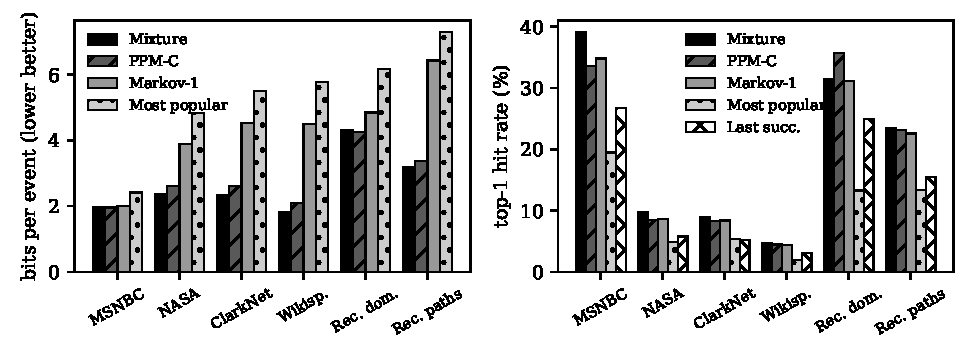
\includegraphics[width=\textwidth]{fig_route0.pdf}
\caption{Route 0, offline replay. Left: log-loss in bits per event. Right: share of events the method ranked first.}
\label{fig:r0}
\end{figure}

\textbf{Route 1.} On the first round, when nothing was cached, Unbound needed a median of \V{r1.cold.unbound_alone.median_ms}\,ms and Unbound with the predictor \V{r1.cold.unbound_plus_predictor.median_ms}\,ms, against \V{r1.cold.system_default.median_ms}\,ms for the campus resolver, which already held most popular names. In later rounds the medians were \V{r1.warm.system_default.median_ms}, \V{r1.warm.unbound_alone.median_ms} and \V{r1.warm.unbound_plus_predictor.median_ms}\,ms; at the 75th percentile, where expired records show, the predictor cut Unbound's \V{r1.warm.unbound_alone.p75_ms}\,ms to \V{r1.warm.unbound_plus_predictor.p75_ms}\,ms [\V{r1.warm.unbound_plus_predictor.p75_ci95.lo}, \V{r1.warm.unbound_plus_predictor.p75_ci95.hi}], but the shared campus resolver stayed fastest at \V{r1.warm.system_default.p75_ms}\,ms (Figure~\ref{fig:r1}).

\begin{figure}[t]
\centering
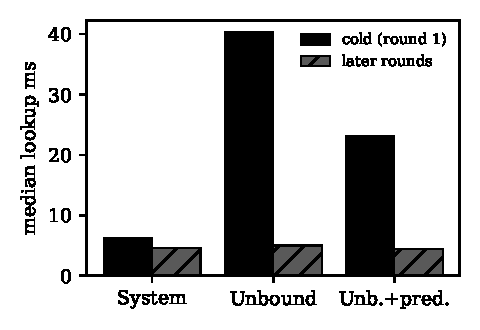
\includegraphics[width=0.55\textwidth]{fig_route1.pdf}
\caption{Route 1, median lookup time for the Tranco top \V{r1.names}.}
\label{fig:r1}
\end{figure}

\textbf{Route 2.} Table~\ref{tab:r2} and Figure~\ref{fig:r2} give the medians for \V{r2.n} measured visits (\V{r2.errors} site failures excluded). The paired extension effect on the wait for the next page was \V{r2.10.eff.ext}\,ms [\V{r2.10.eff.ext.lo}, \V{r2.10.eff.ext.hi}] at 10\,ms, \V{r2.60.eff.ext}\,ms [\V{r2.60.eff.ext.lo}, \V{r2.60.eff.ext.hi}] at 60\,ms and \V{r2.150.eff.ext}\,ms [\V{r2.150.eff.ext.lo}, \V{r2.150.eff.ext.hi}] at 150\,ms (negative is faster). The Mac tool's paired effect on the home page load was \V{r2.10.eff.mac}, \V{r2.60.eff.mac} and \V{r2.150.eff.mac}\,ms at the three profiles.

\begin{table}[t]
\centering\small
\begin{tabular}{lrrrr}
\toprule
 & \multicolumn{2}{c}{Extension off} & \multicolumn{2}{c}{Extension on}\\
Wi-Fi profile & Mac off & Mac on & Mac off & Mac on\\
\midrule
Home, 10 ms & \V{r2.10.off.off.next} & \V{r2.10.off.on.next} & \V{r2.10.on.off.next} & \V{r2.10.on.on.next}\\
Campus, 60 ms & \V{r2.60.off.off.next} & \V{r2.60.off.on.next} & \V{r2.60.on.off.next} & \V{r2.60.on.on.next}\\
Poor, 150 ms & \V{r2.150.off.off.next} & \V{r2.150.off.on.next} & \V{r2.150.on.off.next} & \V{r2.150.on.on.next}\\
\bottomrule
\end{tabular}
\caption{Route 2, median wait for the next page (ms).}
\label{tab:r2}
\end{table}

\begin{figure}[t]
\centering
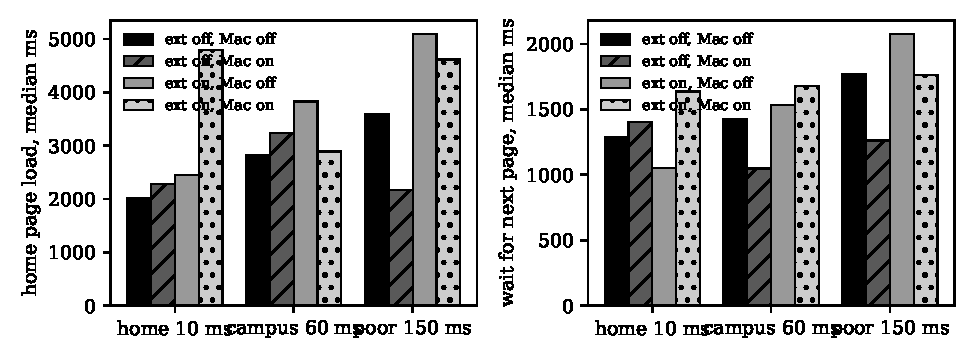
\includegraphics[width=\textwidth]{fig_route2.pdf}
\caption{Route 2 by Wi-Fi profile. Left: home page load. Right: wait for the next page after the click.}
\label{fig:r2}
\end{figure}

\textbf{Route 3.} For API calls in later rounds the Mac tool saved a paired median of \V{r3.warm.paired}\,ms [\V{r3.warm.paired.lo}, \V{r3.warm.paired.hi}] per call ($n=\V{r3.warm.paired.n}$; median total \V{r3.warm.off.total} vs \V{r3.warm.on.total}\,ms). On the first round it cost \V{r3.cold.paired}\,ms [\V{r3.cold.paired.lo}, \V{r3.cold.paired.hi}] ($n=\V{r3.cold.paired.n}$), because a cold local Unbound resolves from the root down while the campus resolver already holds the names.

\section{Benchmarks}
\textbf{Prediction.} Against the four predictors, the mixture had the lowest log-loss on most traces. It lost to PPM-C on bits for the recorded domains (\V{r0.recorded_chrome_domains.mixture.bits} vs \V{r0.recorded_chrome_domains.ppm_c.bits}) and MSNBC (\V{r0.msnbc.mixture.bits} vs \V{r0.msnbc.ppm_c.bits}), and on top-1 for the recorded domains (\V{r0.recorded_chrome_domains.mixture.top1}\% vs \V{r0.recorded_chrome_domains.ppm_c.top1}\%).

\textbf{Pages.} At 60\,ms, with a person who hovers 300\,ms before clicking, the median wait for the next page was \V{pb.default.med}\,ms with Chrome's default ($n=\V{pb.default.n}$), \V{pb.instantpage.med}\,ms with instant.page ($n=\V{pb.instantpage.n}$), \V{pb.quicklink.med}\,ms with Quicklink ($n=\V{pb.quicklink.n}$) and \V{pb.extension.med}\,ms with this extension ($n=\V{pb.extension.n}$). Quicklink made \V{pb.quicklink.spec} speculative requests to serve its hits; the extension made \V{pb.extension.spec}. This benchmark covers only the sites finished in the time available, so its intervals are wide (see \texttt{RESULTS.md}).

\textbf{Lookups.} Against plain Unbound, the predictor lowered both the cold median and the warm 75th percentile (Route 1). Against the network's own resolver it did not: a shared campus resolver serves popular names from a cache filled by thousands of users.

\section{Limitations}
All timing comes from one Mac on one campus network over one evening; a home network with a slow or distant resolver would favour the Mac tool more, and the campus result likely understates it. Route 2's training is one visit per site, far less history than a person builds, and its sites are the most popular on the web. The Safari arm of Route 2, the live check on the author's own Mac and Chrome, and installation with real port-53 DNS settings need an administrator password and were not run unattended; the macOS safety behaviours were tested with real Unbound and simulated system tools. The page benchmark's $n$ is small. The extension's last-write-wins storage can lose an update when two tabs of one site navigate at the same instant.
